% =============================================================================
% ACE: Active Causal Experimentalist
% Conference talk slides (~20 slides)
% Compile: pdflatex slides.tex   (requires metropolis Beamer theme)
% =============================================================================
\documentclass[aspectratio=169,10pt]{beamer}
\usetheme{metropolis}
\usepackage{tikz}
\usetikzlibrary{arrows.meta,positioning,shapes.geometric,calc}
\usepackage{amsmath,amssymb,mathtools,bbm}
\usepackage{booktabs}
\usepackage{xcolor}

% Pull figures from the paper directory; place slide-specific figures in ./figs
\graphicspath{{../paper/figs/}{./figs/}}

% Operator
\DeclareMathOperator*{\argmax}{arg\,max}

% Lightweight citation stubs for slides (avoids natbib in beamer).
\providecommand{\citet}[1]{}
\providecommand{\citep}[1]{}

% A bit of color discipline shared with the paper
\definecolor{ACEred}{rgb}{0.70,0.00,0.00}
\definecolor{slategray}{rgb}{0.35,0.40,0.50}

\title{Active Causal Experimentalist (ACE)}
\subtitle{Learning Intervention Strategies via Direct Preference Optimization}
\date{NeurIPS 2026}
\author{Anonymous Authors}
\institute{}

\begin{document}

% --------------- 1. TITLE ---------------------------------------------------
\maketitle

% --------------- 2. THE QUESTION --------------------------------------------
\begin{frame}{Sequential decisions in causal experiments}
\begin{itemize}
  \item Testing 100 candidate compounds pairwise: 4{,}950 experiments.
  \item A 10-component alloy at 5 temperatures: $5^{10}$ configurations.
  \item Modern simulators expose hundreds of interacting variables.
\end{itemize}
\vspace{0.4em}
\textbf{Question.} Each intervention reveals information that should inform the
next one. \emph{Where do you intervene first, and how does the answer change as you learn?}
\vspace{0.4em}
\begin{itemize}
  \item Random sampling, round-robin coverage, and greedy info-gain treat each
        decision in isolation.
  \item No transfer of insight across systems; no adaptation as knowledge accumulates.
\end{itemize}
\end{frame}

% --------------- 3. PEARL'S CAUSAL HIERARCHY --------------------------------
\begin{frame}{Pearl's causal hierarchy: we live at Rung 2}
\begin{columns}[T,onlytextwidth]
\column{0.45\textwidth}
\centering
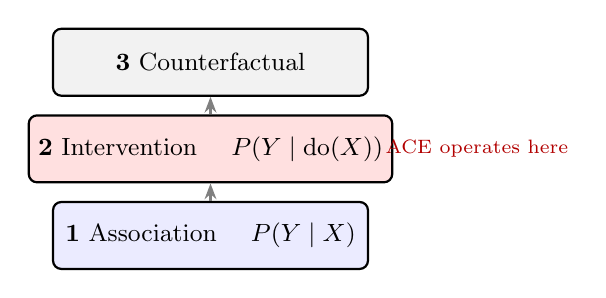
\begin{tikzpicture}[
    rung/.style={draw, thick, minimum width=4.0cm, minimum height=0.85cm, font=\small, rounded corners=3pt},
    arrow/.style={-{Stealth[length=2mm]}, thick, gray}
]
\node[rung, fill=blue!8] (r1) at (0,0)   {\textbf{1} Association \quad $P(Y\mid X)$};
\node[rung, fill=red!12]  (r2) at (0,1.1) {\textbf{2} Intervention \quad $P(Y\mid \text{do}(X))$};
\node[rung, fill=gray!10] (r3) at (0,2.2) {\textbf{3} Counterfactual};
\draw[arrow] (r1) -- (r2);
\draw[arrow] (r2) -- (r3);
\node[font=\scriptsize, ACEred, anchor=west] at (2.1,1.1) {ACE operates here};
\end{tikzpicture}
\column{0.55\textwidth}
\small
Reichenbach's common cause: any $A \perp\!\!\!\!\not\perp B$ in observational data
is consistent with $A\!\to\!B$, $B\!\to\!A$, or $A\!\leftarrow\!C\!\rightarrow\!B$.
\smallskip
\begin{itemize}
  \item Observational data alone cannot identify mechanisms beyond the Markov equivalence class.
  \item Only Rung-2 interventions $\text{do}(V_i\!=\!\nu)$ break the symmetry.
  \item Eberhardt: $n\!-\!1$ interventions suffice; adaptive strategies beat non-adaptive.
\end{itemize}
\end{columns}
\end{frame}

% --------------- 4. MECHANISM ESTIMATION SETTING ----------------------------
\begin{frame}{Setting: mechanism estimation given the graph}
\begin{itemize}
  \item SCM $\mathcal{M}=\langle\mathcal{U},\mathcal{V},\mathcal{F},P(\mathcal{U})\rangle$, with
        $V_i = f_i(\text{Pa}_i, U_i)$.
  \item Graph $\mathcal{G}$ \emph{given}; recover $\{f_i\}$ from sequential interventions.
  \item Two interacting components:
        \begin{itemize}
          \item Environment $M^*$: oracle SCM, returns samples under $\text{do}(V_i\!=\!\nu)$.
          \item Learner $M_\theta$: parametric estimate, MLP per non-root node.
        \end{itemize}
\end{itemize}
\vspace{0.3em}
\textbf{Why not joint structure-and-mechanism learning?}
\begin{itemize}
  \item ABCI / CBED maintain DAG posteriors: combinatorial in $|V|$.
  \item Largest published evaluation reaches $\sim$20 nodes.
  \item Known structure is what enables the 30-node regime ACE targets.
\end{itemize}
\end{frame}

% --------------- 5. ACE FRAMEWORK -------------------------------------------
\begin{frame}{The ACE framework}
\centering
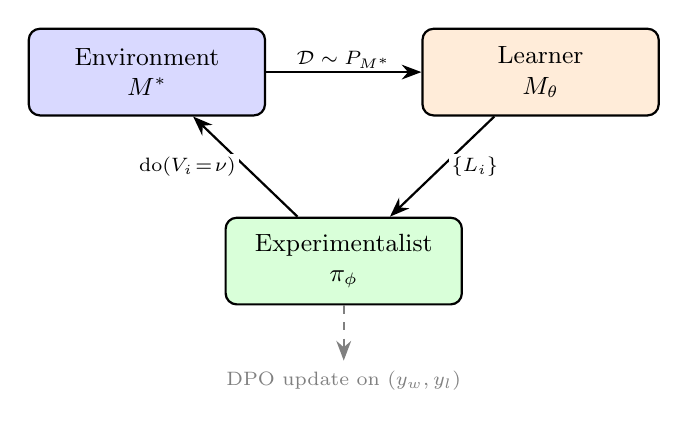
\begin{tikzpicture}[
    box/.style={rectangle, draw, rounded corners, minimum width=3.0cm,
                minimum height=1.1cm, font=\small, thick, align=center},
    env/.style={box, fill=blue!15},
    learn/.style={box, fill=orange!15},
    agent/.style={box, fill=green!15},
    arrow/.style={-{Stealth[length=2.5mm]}, thick},
    label/.style={font=\scriptsize, midway, fill=white, inner sep=1pt}
]
\node[env]   (env)   at (0,0)    {Environment\\$M^*$};
\node[learn] (learn) at (5.0,0)  {Learner\\$M_\theta$};
\node[agent] (agent) at (2.5,-2.4) {Experimentalist\\$\pi_\phi$};
\draw[arrow] (agent) -- node[label, left, xshift=-2pt] {$\text{do}(V_i\!=\!\nu)$} (env);
\draw[arrow] (env)   -- node[label, above] {$\mathcal{D}\sim P_{M^*}$} (learn);
\draw[arrow] (learn) -- node[label, right, xshift=2pt] {$\{L_i\}$} (agent);
\draw[arrow, dashed, gray] (agent.south) -- ++(0,-0.7)
      node[below, font=\scriptsize, gray] {DPO update on $(y_w,y_l)$};
\end{tikzpicture}
\vspace{0.2em}
\begin{itemize}
\item Environment $\to$ data; learner $\to$ per-node losses; experimentalist $\to$ next intervention.
\item Loop closes via DPO: best vs.\ worst candidate becomes a preference pair.
\end{itemize}
\end{frame}

% --------------- 6. ALGORITHM STEP ------------------------------------------
\begin{frame}{One ACE step}
\begin{columns}[T,onlytextwidth]
\column{0.55\textwidth}
\centering
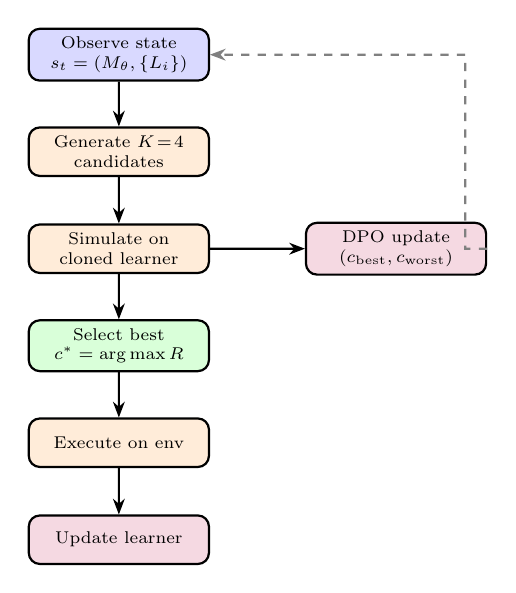
\begin{tikzpicture}[
    scale=0.88, transform shape,
    box/.style={rectangle, draw, rounded corners,
                minimum width=2.6cm, minimum height=0.7cm,
                font=\scriptsize, thick, align=center},
    state/.style={box, fill=blue!15},
    process/.style={box, fill=orange!15},
    decision/.style={box, fill=green!15},
    update/.style={box, fill=purple!15},
    arrow/.style={-{Stealth[length=2mm]}, thick}
]
\node[state]    (s)    at (0,0)    {Observe state\\$s_t = (M_\theta,\{L_i\})$};
\node[process]  (g)    at (0,-1.4) {Generate $K\!=\!4$\\candidates};
\node[process]  (sim)  at (0,-2.8) {Simulate on\\cloned learner};
\node[decision] (sel)  at (0,-4.2) {Select best\\$c^*=\argmax R$};
\node[process]  (e)    at (0,-5.6) {Execute on env};
\node[update]   (l)    at (0,-7.0) {Update learner};
\node[update]   (dpo)  at (4.0,-2.8) {DPO update\\$(c_\text{best},c_\text{worst})$};
\foreach \a/\b in {s/g, g/sim, sim/sel, sel/e, e/l} {\draw[arrow] (\a) -- (\b);}
\draw[arrow] (sim) -- (dpo);
\draw[arrow, dashed, gray] (dpo) -- ++(1.0,0) |- (s.east);
\end{tikzpicture}
\column{0.45\textwidth}
\small
\textbf{Five steps each episode:}
\begin{enumerate}
\item Read graph + per-node losses + recent history into a text prompt.
\item LM emits $K=4$ candidate $\text{do}(V_i\!=\!\nu)$.
\item Lookahead: each candidate runs on a cloned learner.
\item Execute the best; learner ingests the new data.
\item DPO update: $(\text{best},\text{worst})$ pair refines the policy.
\end{enumerate}
\smallskip
\textit{One preference pair per intervention; preference data scales with experiments.}
\end{columns}
\end{frame}

% --------------- 7. THE COMPOSITE REWARD ------------------------------------
\begin{frame}{The composite reward}
\[
R(c,\sigma) \;=\; \underbrace{\Delta\mathcal{L}}_{\text{information gain}}
                  \;+\; \alpha\!\cdot\!\underbrace{w(V_i,\{L_j\})}_{\text{node importance}}
                  \;+\; \gamma\!\cdot\!\underbrace{D(V_i,H)}_{\text{diversity}}
\]
\begin{itemize}
\item $\Delta\mathcal{L} = L_\text{before}\!-\!L_\text{after}$, the loss reduction estimated by lookahead.
\item $w$ upweights nodes with high current loss \emph{and} few recent interventions:
  \[ w(V_i,\{L_j\})=\texttt{cov\_bonus}\cdot\tfrac{L_i}{\sum_j L_j}\cdot(1+n_i(H))^{-1/2}.\]
\item $D$ penalizes concentration on already-sampled nodes / values.
\end{itemize}
\smallskip
Default weights: $\alpha=0.1$, $\gamma=0.05$. $\Delta\mathcal{L}$ stays dominant
($\sim$80--90\%); ablation shows $\gamma\!>\!0$ is critical, $\alpha$ has wide stable range.
\end{frame}

% --------------- 8. WHY A LANGUAGE MODEL? -----------------------------------
\begin{frame}{Why a language model?}
\textbf{Active design at Rung 2 needs a forward model.} Quality of policy is bounded by
quality of forward-model prior.
\smallskip
\begin{itemize}
\item \textbf{MLP from scratch.} Uniform prior; must construct the forward model from
      experience, episode by episode, within a fixed budget.
\item \textbf{One-step Bayesian acquisition (Bayesian OED).} Correct but \emph{shallow}:
      cannot reason about multi-step strategies like ``first resolve $X_2$ to unlock the
      $X_3$ collider.''
\item \textbf{Pretrained LM.} Encodes a \emph{deep} but uncalibrated prior over how
      variables in real systems relate causally. Scientific corpora are full of
      Rung-2 statements (``clamping $X_2$ breaks the synchronization''),
      and these statements raise $\log\pi$ on the corresponding interventions.
\end{itemize}
\smallskip
DPO supplies the calibration. The LM provides breadth; DPO provides specificity.
\end{frame}

% --------------- 9. LM AS WORLD MODEL ---------------------------------------
\begin{frame}{The LM as a contextual world model}
\begin{itemize}
\item \textbf{K\i c\i man et al.\ 2023:} GPT-4 well above chance on pairwise causal-direction
      benchmarks; the prior is real, not pattern-matching.
\item \textbf{Hao et al.\ 2023 (RAP):} LM as both reasoner and world-model in a
      planning loop. ACE realizes this dual role per intervention step.
\item \textbf{Xie et al.\ 2022:} in-context learning $=$ implicit Bayesian inference
      under the pretraining prior. Prompt encodes the agent's epistemic state;
      generation is an approximate posterior predictive.
\end{itemize}
\smallskip
\textbf{Practical consequences for ACE:}
\begin{itemize}
\item Variable-size action $(V_i,\nu)$ handled natively by token generation.
\item Same weights transfer across 5- and 30-node SCMs, Duffing, and economic data.
\item $\log\pi(y\mid x)$ exact, which is what DPO requires.
\end{itemize}
\smallskip
\footnotesize\textit{Claim is narrow: LMs provide a better starting point than uniform / greedy
priors. DPO does the calibration to the specific system.}
\end{frame}

% --------------- 10. DPO OBJECTIVE ------------------------------------------
\begin{frame}{Direct Preference Optimization}
\textbf{Preferences are not human-provided.} They come from the reward $R$ on
simulated outcomes (RLAIF): per step, the highest-reward candidate $y_w$ wins
over the lowest $y_l$.
\[
\mathcal{L}_\text{DPO} \;=\; -\mathbb{E}_{(y_w,y_l)}
   \log\sigma\!\left(\beta
   \left[\log\tfrac{\pi_\phi(y_w)}{\pi_\text{ref}(y_w)}
        - \log\tfrac{\pi_\phi(y_l)}{\pi_\text{ref}(y_l)}\right]\right).
\]
\begin{itemize}
\item $\beta=0.1$, $\pi_\text{ref}$ updated every 25 episodes.
\item Loss depends on \emph{log-probability ratios}, not absolute reward magnitudes.
\item This decouples training from the reward scale, the property we exploit next.
\end{itemize}
\end{frame}

% --------------- 11. THEORY -------------------------------------------------
\begin{frame}{Theory: scale invariance of preference learning}
\textbf{Assumption.} \emph{Decomposable diminishing reward.}
$r_t(a) = f(t)\cdot g(a)$ with $f$ positive and non-increasing; $g$ approximately stationary.
\medskip

\textbf{Proposition.}
\begin{enumerate}
\item \emph{Preference invariance.} $r_t(a_w)\!>\!r_t(a_l)$ for all $t$ whenever $g(a_w)\!>\!g(a_l)$.
\item \emph{Value non-stationarity.} $V_t(s)=f(t)\cdot\mathbb{E}_a[g(a)\mid s]$ scales with $f(t)$.
\item \emph{DPO invariance.} $\nabla_\phi \mathcal{L}_\text{DPO}$ is invariant to multiplicative
      rescaling of all rewards.
\end{enumerate}
\medskip

\textbf{Empirical support.} $\mathbb{E}[\Delta\mathcal{L}]$ drops $\sim\!500\times$ between
early and late training, while candidate-rank Spearman $\rho$ stays $>0.85$ throughout.
\end{frame}

% --------------- 12. WHY PPO STRUGGLES --------------------------------------
\begin{frame}{Why DPO beats value-based RL empirically}
\centering
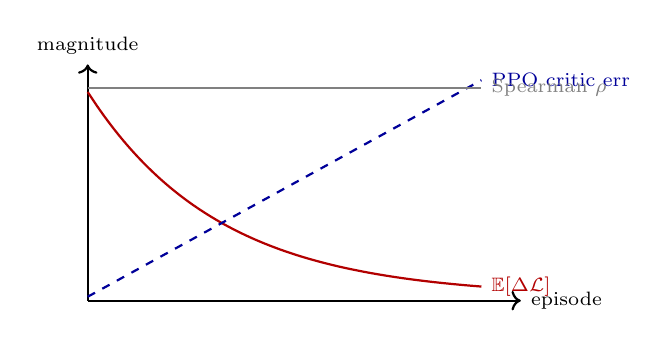
\begin{tikzpicture}
\begin{scope}
\draw[->,thick] (0,0) -- (5.5,0) node[right, font=\scriptsize] {episode};
\draw[->,thick] (0,0) -- (0,3.0) node[above, font=\scriptsize] {magnitude};
\draw[ACEred, thick]      plot[smooth, samples=50, domain=0:5] (\x, {2.6*exp(-0.6*\x) + 0.05}) node[right, font=\scriptsize, ACEred] {$\mathbb{E}[\Delta\mathcal{L}]$};
\draw[blue!60!black, thick, dashed] plot[smooth, samples=50, domain=0:5] (\x, {0.05 + 0.55*\x}) node[right, font=\scriptsize, blue!60!black] {PPO critic err};
\draw[gray, thick]        plot[smooth, samples=50, domain=0:5] (\x, {2.7}) node[right, font=\scriptsize, gray] {Spearman $\rho$};
\end{scope}
\end{tikzpicture}
\medskip
\begin{itemize}
\item ACE outperforms PPO by $70\%$ at \emph{identical reward signals}.
\item PPO's critic accumulates value-prediction error from $0.02$ (early) $\to$ $3.8$ (late).
\item DPO sidesteps the magnitude collapse: log-ratios are scale-invariant
      (Proposition).
\end{itemize}
\end{frame}

% --------------- 13. EXPERIMENTAL SETUP -------------------------------------
\begin{frame}{Experimental setup}
\textbf{Domains.}
\begin{itemize}
\item 5-node synthetic SCM (controlled diagnostic; collider, nonlinearity, disconnected component).
\item 30-node hierarchical SCM (scaling test).
\item Coupled Duffing oscillators (physics).
\item Phillips Curve / FRED macroeconomic data (active data subset selection; appendix).
\end{itemize}
\smallskip
\textbf{Baselines.} Random; Round-Robin (Fisher 1935);
Max-Variance (Cohn et al.\ 1996); Bayesian OED (Monte Carlo EIG, adapted from
Toth et al.\ 2022 / Tigas et al.\ 2022); PPO (Schulman et al.\ 2017).
\smallskip
\textbf{Seed counts.} ACE 5-node N=5; ACE 30-node N=3; baselines + PPO N=5;
Bayesian OED N=3 (higher per-seed compute). All methods on the same MLP student
learner for fairness.
\end{frame}

% --------------- 14. 5-NODE BENCHMARK ---------------------------------------
\begin{frame}{5-node synthetic benchmark}
\begin{columns}[T,onlytextwidth]
\column{0.5\textwidth}
\centering
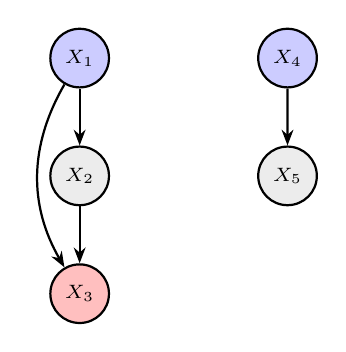
\begin{tikzpicture}[
    scale=0.88,
    root/.style={circle, draw, fill=blue!20, minimum size=0.7cm, font=\scriptsize, thick},
    regular/.style={circle, draw, fill=gray!15, minimum size=0.7cm, font=\scriptsize, thick},
    collider/.style={circle, draw, fill=red!25, minimum size=0.7cm, font=\scriptsize, thick},
    arrow/.style={-{Stealth[length=2mm]}, thick}
]
\node[root]    (X1) at (0,0)     {$X_1$};
\node[root]    (X4) at (3.0,0)   {$X_4$};
\node[regular] (X2) at (0,-1.7)  {$X_2$};
\node[regular] (X5) at (3.0,-1.7){$X_5$};
\node[collider](X3) at (0,-3.4)  {$X_3$};
\draw[arrow] (X1) -- (X2);
\draw[arrow] (X2) -- (X3);
\draw[arrow] (X1) to[bend right=30] (X3);
\draw[arrow] (X4) -- (X5);
\end{tikzpicture}
\column{0.5\textwidth}
\small
\textbf{What it tests.}
\begin{itemize}
\item Collider identification: $X_3$ with parents $X_1,X_2$ and nonlinear $\sin$.
\item Mixed mechanism types: linear ($X_2$), nonlinear+trig ($X_3$), quadratic ($X_5$).
\item Disconnected components: $X_4\to X_5$ unrelated to the collider.
\end{itemize}
\smallskip
\textit{Diagnostic testbed, not the headline. The 30-node and Duffing
results carry the scaling and transfer story.}
\end{columns}
\end{frame}

% --------------- 15. 5-NODE RESULTS -----------------------------------------
\begin{frame}{5-node results}
\centering
\small
\begin{tabular}{@{}lccc@{}}
\toprule
Method (171 ep.) & Mean$\pm$Std & Median & Improvement \\
\midrule
\textbf{ACE (DPO)} & \textbf{0.92$\pm$0.73} & \textbf{0.61} & --- \\
\midrule
Random         & 2.17$\pm$0.07 & 2.21 & 72\% \\
Round-Robin    & 2.10$\pm$0.11 & 2.09 & 71\% \\
Max-Variance   & 2.11$\pm$0.14 & 2.10 & 71\% \\
Bayesian OED   & 2.04$\pm$0.12 & 1.99 & 69\% \\
PPO            & 2.08$\pm$0.06 & 2.06 & 70\% \\
\bottomrule
\end{tabular}
\vspace{0.5em}
\begin{itemize}
\item All baselines plateau in $[2.04, 2.17]$. Bayesian OED is the strongest of them.
\item ACE median: $0.61$, a $69\%$ improvement over Bayesian OED at matched budget.
\item Improvement isolates \emph{learned multi-step strategy} beyond one-step EIG.
\end{itemize}
\end{frame}

% --------------- 16. 30-NODE SCM STRUCTURE ----------------------------------
\begin{frame}[fragile]{30-node hierarchical SCM}
\centering
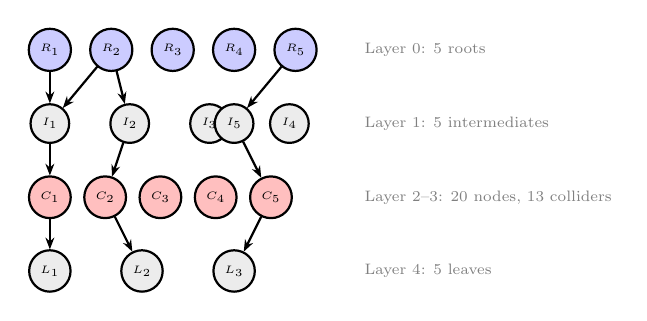
\begin{tikzpicture}[
    scale=0.78, transform shape,
    root/.style={circle, draw, fill=blue!20, minimum size=0.5cm, font=\tiny, thick},
    regular/.style={circle, draw, fill=gray!15, minimum size=0.5cm, font=\tiny, thick},
    collider/.style={circle, draw, fill=red!25, minimum size=0.5cm, font=\tiny, thick},
    arrow/.style={-{Stealth[length=1.5mm]}, thick}
]
% Layer 0
\node[root] (r1) at (0,0)   {$R_1$};
\node[root] (r2) at (1.0,0) {$R_2$};
\node[root] (r3) at (2.0,0) {$R_3$};
\node[root] (r4) at (3.0,0) {$R_4$};
\node[root] (r5) at (4.0,0) {$R_5$};
% Layer 1
\node[regular] (i1) at (0,-1.2)   {$I_1$};
\node[regular] (i2) at (1.3,-1.2) {$I_2$};
\node[regular] (i3) at (2.6,-1.2) {$I_3$};
\node[regular] (i4) at (3.9,-1.2) {$I_4$};
\node[regular] (i5) at (3.0,-1.2) {$I_5$};
% Layer 2--3 (representative)
\node[collider] (c1) at (0,-2.4)   {$C_1$};
\node[collider] (c2) at (0.9,-2.4) {$C_2$};
\node[collider] (c3) at (1.8,-2.4) {$C_3$};
\node[collider] (c4) at (2.7,-2.4) {$C_4$};
\node[collider] (c5) at (3.6,-2.4) {$C_5$};
% Layer 4
\node[regular] (l1) at (0,-3.6)   {$L_1$};
\node[regular] (l2) at (1.5,-3.6) {$L_2$};
\node[regular] (l3) at (3.0,-3.6) {$L_3$};
% Edges (representative)
\draw[arrow] (r1) -- (i1);
\draw[arrow] (r2) -- (i1);
\draw[arrow] (r2) -- (i2);
\draw[arrow] (r5) -- (i5);
\draw[arrow] (i1) -- (c1);
\draw[arrow] (i2) -- (c2);
\draw[arrow] (i5) -- (c5);
\draw[arrow] (c1) -- (l1);
\draw[arrow] (c2) -- (l2);
\draw[arrow] (c5) -- (l3);
% Layer captions
\node[font=\scriptsize, gray, anchor=west] at (5.0,0)    {Layer 0: 5 roots};
\node[font=\scriptsize, gray, anchor=west] at (5.0,-1.2) {Layer 1: 5 intermediates};
\node[font=\scriptsize, gray, anchor=west] at (5.0,-2.4) {Layer 2--3: 20 nodes, 13 colliders};
\node[font=\scriptsize, gray, anchor=west] at (5.0,-3.6) {Layer 4: 5 leaves};
\end{tikzpicture}
\smallskip
\begin{itemize}
\item 30 nodes, 39 edges, 11 colliders. Five-layer hierarchy.
\item Random sampling devotes only $\sim\!3.3\%$ of interventions per node.
\end{itemize}
\end{frame}

% --------------- 17. 30-NODE RESULTS (HEADLINE) -----------------------------
\begin{frame}{30-node results: the headline}
\centering

\includegraphics[width=0.95\textwidth]{fig_30node_results.pdf}
\vspace{0.3em}
\begin{itemize}
\item ACE descends to best-loss $\mathbf{1.95\pm 0.77}$; baselines plateau at $\mathbf{5.86}$ (stds $<0.08$).
\item All three passive baselines indistinguishable: at scale, static heuristics cannot differentiate themselves.
\item $\mathbf{3.0\times}$ improvement, robust to seed selection (stable-seed mean: $1.54$).
\end{itemize}
\end{frame}

% --------------- 18. DUFFING ------------------------------------------------
\begin{frame}{Coupled Duffing oscillators: Rung-2 in physics}
\begin{columns}[T,onlytextwidth]
\column{0.42\textwidth}
\centering
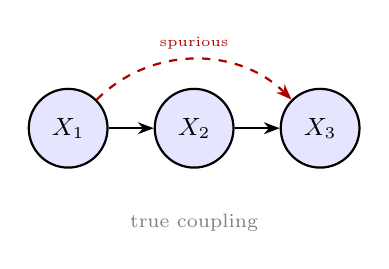
\begin{tikzpicture}[
    scale=1.0,
    osc/.style={circle, draw, fill=blue!10, minimum size=1.0cm, font=\small, thick},
    arrow/.style={-{Stealth[length=2mm]}, thick}
]
\node[osc] (X1) at (0,0)   {$X_1$};
\node[osc] (X2) at (1.6,0) {$X_2$};
\node[osc] (X3) at (3.2,0) {$X_3$};
\draw[arrow] (X1) -- (X2);
\draw[arrow] (X2) -- (X3);
\draw[arrow, dashed, ACEred] (X1) to[bend left=45] node[above, font=\tiny, ACEred] {spurious} (X3);
\node[font=\scriptsize, gray] at (1.6,-1.2) {true coupling};
\end{tikzpicture}
\column{0.58\textwidth}
\small
\textbf{Coupling-parameter MSE} (N=5, 100 episodes):
\medskip
\begin{tabular}{@{}lcc@{}}
\toprule
Method & Error & vs.\ Random \\
\midrule
\textbf{ACE} & \textbf{0.042$\pm$0.036} & $5.8\times$ \\
Round-Robin  & 0.238$\pm$0.076 & $1.0\times$ \\
Random       & 0.245$\pm$0.121 & --- \\
\bottomrule
\end{tabular}
\medskip
\textbf{Strategy.} ACE puts $\mathbf{62\%}$ of interventions on $X_2$ (the
intermediate), clamping it to break the synchronization-induced
$X_1\!\leftrightarrow\!X_3$ correlation. Discovered autonomously, no instruction.
\end{columns}
\end{frame}

% --------------- 19. COMPONENT ABLATION -------------------------------------
\begin{frame}{Component ablation}
\centering
\small
\begin{tabular}{@{}lcc@{}}
\toprule
Configuration & Total Loss & Failure mode \\
\midrule
ACE (full)                        & $0.92\pm0.73$  & --- \\
\midrule
No DPO (random proposals + lookahead) & $2.10\pm0.11$ & no learned strategy \\
No per-node convergence (fixed 100 ep.)& $1.45\pm0.62$ & early termination \\
No dedicated root learner             & $1.38\pm0.55$ & root distribution failure \\
No diversity reward                   & $2.82\pm0.22$ & node collapse \\
\bottomrule
\end{tabular}
\vspace{0.5em}
\begin{itemize}
\item \textbf{Diversity reward is critical}: without it, the policy over-concentrates and
      \emph{worsens} beyond every passive baseline.
\item \textbf{Lookahead alone is not enough}: random candidates with selection match Round-Robin.
      Learned proposal generation is essential.
\end{itemize}
\end{frame}

% --------------- 20. EMERGENT STRATEGY --------------------------------------
\begin{frame}[fragile]{Emergent strategy: collider concentration}
\begin{columns}[T,onlytextwidth]
\column{0.45\textwidth}
\centering
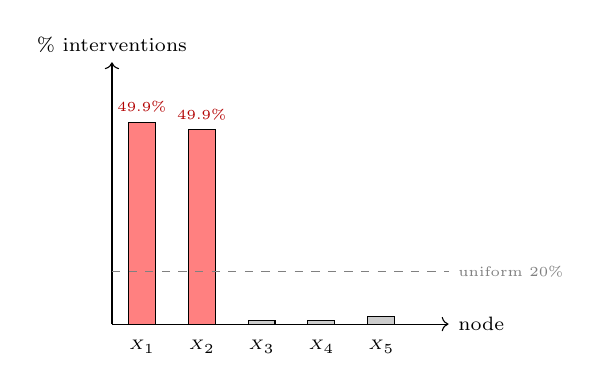
\begin{tikzpicture}[scale=0.95]
\draw[->] (0,0) -- (4.5,0) node[right, font=\scriptsize] {node};
\draw[->] (0,0) -- (0,3.5) node[above, font=\scriptsize] {\% interventions};
% bars
\filldraw[fill=red!50, draw=black, thin]  (0.22,0) rectangle (0.58,2.7);
\filldraw[fill=red!50, draw=black, thin]  (1.02,0) rectangle (1.38,2.6);
\filldraw[fill=gray!40, draw=black, thin] (1.82,0) rectangle (2.18,0.05);
\filldraw[fill=gray!40, draw=black, thin] (2.62,0) rectangle (2.98,0.05);
\filldraw[fill=gray!40, draw=black, thin] (3.42,0) rectangle (3.78,0.10);
% labels
\node[font=\tiny] at (0.40,-0.3) {$X_1$};
\node[font=\tiny] at (1.20,-0.3) {$X_2$};
\node[font=\tiny] at (2.00,-0.3) {$X_3$};
\node[font=\tiny] at (2.80,-0.3) {$X_4$};
\node[font=\tiny] at (3.60,-0.3) {$X_5$};
% reference line
\draw[gray, dashed] (0,0.7) -- (4.5,0.7) node[right, font=\tiny, gray] {uniform 20\%};
\node[font=\tiny, ACEred, anchor=south] at (0.40,2.7) {49.9\%};
\node[font=\tiny, ACEred, anchor=south] at (1.20,2.6) {49.9\%};
\end{tikzpicture}
\column{0.55\textwidth}
\small
\begin{itemize}
\item ACE concentrates $\mathbf{99.8\%}$ of interventions on $X_1, X_2$
      (the parents of the collider $X_3$).
\item \textbf{Causal-theoretic optimum}: identifying $f_3$ requires varying
      both parents independently.
\item \textbf{Cross-seed consistency:} per-node intervention-fraction std
      is $<\!0.01$ for $X_1, X_2$. Strategy is robust to seed.
\item Bayesian OED, with explicit one-step EIG, plateaus at $2.04$.
      ACE's median is $0.61$ on the same budget.
\item The strategy was \emph{not} engineered. It emerged from preference
      optimization over the composite reward.
\end{itemize}
\end{columns}
\end{frame}

% --------------- 21. LIMITATIONS & CONCLUSION -------------------------------
\begin{frame}{Limitations and conclusion}
\textbf{Limitations.}
\begin{itemize}
\item Known structure: ABCI/CBED jointly learn structure but operate $\le 20$ nodes;
      ACE is the natural mechanism-estimation half of a pipeline.
\item Text-based encoding limits scaling beyond $\sim 50$ nodes; GNN policies are next.
\item Compute: $\sim 22$ min/step on A100, $\sim 6$--$8$ h per seed.
\item Oracle pretraining ($200$ interventions) accelerates but does not fundamentally
      enable the strategy.
\end{itemize}
\medskip
\textbf{Three contributions.}
\begin{enumerate}
\item \emph{Empirical:} $55\%$ over Bayesian OED (5-node), $3.0\times$ over the baseline
      plateau (30-node), $5.8\times$ on Duffing.
\item \emph{Theoretical:} scale-invariance of preference learning under diminishing rewards
      (Proposition).
\item \emph{Emergent:} $99.8\%$ concentration on collider parents, recovered autonomously.
\end{enumerate}
\end{frame}

% --------------- 22. THANK YOU ----------------------------------------------
\begin{frame}[standout]
Questions?
\medskip\\
\small
ACE: experimental design as a learnable policy,\\
trained by Direct Preference Optimization,\\
with a pretrained LM as contextual forward model.
\end{frame}

\end{document}
